\documentclass[handout]{beamer}
%==============================================================
% Common Beamer Preamble for Course Lectures: Training and Scaling Language Models
%==============================================================

\usepackage[utf8]{inputenc}
\usepackage[T1]{fontenc}
\usepackage{hyperref}
\pdfstringdefDisableCommands{%
  \def\translate#1{#1}%
}
\usepackage{amsmath,amssymb,xcolor,multicol,booktabs,colortbl}
\usepackage{graphicx,listings}
\renewcommand{\figurename}{Figure.}
\renewcommand{\tablename}{Table.}

% ---- TikZ Libraries ----
\usepackage{tikz}
\usetikzlibrary{positioning,arrows.meta,shapes.geometric,calc,fit,backgrounds,decorations.pathreplacing}
\tikzset{
  >={Stealth[length=4pt,width=3pt]},
  every picture/.append style={>={Stealth[length=4pt,width=3pt]}}
}

% ---- Presentation defaults ----
\setbeamertemplate{navigation symbols}{}
\setbeamersize{text margin left=0.55cm,text margin right=0.55cm}
\setbeamerfont{title}{size=\LARGE,series=\bfseries}
\setbeamerfont{subtitle}{size=\large}

% ---- FontAwesome fallback ----
\IfFileExists{fontawesome5.sty}{%
  \usepackage{fontawesome5}%
}{%
  \providecommand{\faMicrochip}{}%
  \providecommand{\faComments}{}%
  \providecommand{\faTools}{}%
  \providecommand{\faCheckCircle}{}%
  \providecommand{\faExclamationTriangle}{}%
  \providecommand{\faImage}{}%
  \providecommand{\faRobot}{}%
  \providecommand{\faTerminal}{}%
  \providecommand{\faBook}{}%
  \providecommand{\faRedo}{}%
  \providecommand{\faLayerGroup}{}%
  \providecommand{\faCogs}{}%
  \providecommand{\faDatabase}{}%
  \providecommand{\faHdd}{}%
  \providecommand{\faNetworkWired}{}%
}

% ---- Theme Style and Semantic Colors ----
%==============================================================
% Centralized Semantic Color Definitions for LLMs Presentation
%==============================================================

% ---- Base Template / Theme Colors (Aligned with Palette B) ----
\definecolor{themenavy}{RGB}{22,70,102}       % Palette B primary cerulean: #164666
\definecolor{themeblue}{RGB}{22,70,102}       % Primary alias
\definecolor{primarylight}{RGB}{34,92,132}    % Primary light: #225c84
\definecolor{themeteal}{RGB}{0,159,176}       % Accent cyan-teal: #009fb0
\colorlet{main_color}{themenavy}
\colorlet{accent}{themeteal}

\definecolor{accentdark}{RGB}{0,108,120}      % Deep cyan-teal for contrast text
\definecolor{accentlight}{RGB}{56,178,214}    % Slate accent cyan: #38b2d6
\definecolor{leafred}{RGB}{197,93,61}         % Terracotta red for branches/leaves

% ---- Website Panel & Border Neutrals ----
\definecolor{panelbg}{RGB}{237,245,249}       % Course-panel: #edf5f9
\definecolor{panelborder}{RGB}{204,226,238}   % Course-border: #cce2ee

% ---- Code listing style (syntax highlights) ----
\definecolor{deepblue}{RGB}{22,70,102}
\definecolor{deepred}{rgb}{0.6,0,0}
\definecolor{deepgreen}{RGB}{0,135,150}
\definecolor{halfgray}{gray}{0.55}

% ---- Semantic Theme Navy / Cerulean Shades ----
\colorlet{themebluebg}{panelbg}               % Panel #edf5f9
\colorlet{themebluecard}{main_color!8}        % Mild card background fills
\colorlet{themeblueborder}{panelborder}       % Border #cce2ee
\colorlet{themebluemid}{themeteal!60}         % Accent mid-contrast
\colorlet{themebluedraw}{main_color!80}       % Strong outline draws/strokes

% ---- Semantic Secondary Accent Teal Shades ----
\colorlet{accentdarkbg}{themeteal!10}        % Light secondary background fills
\colorlet{accentdarkdraw}{themeteal}         % Secondary outlines/strokes/text/axes

% ---- Functional Colors: Success Green ----
\definecolor{successgreen}{RGB}{55,145,55}
\colorlet{successbg}{successgreen!8}
\colorlet{successdraw}{successgreen!75}

% ---- Functional Colors: Alert Red ----
\definecolor{alertred}{RGB}{197,55,55}
\colorlet{alertbg}{alertred!8}
\colorlet{alertdraw}{alertred!75}

% ---- Functional Colors: Warning Orange ----
\definecolor{warningorange}{RGB}{220,110,30}
\colorlet{warningbg}{warningorange!10}
\colorlet{warningdraw}{warningorange!80}

% ---- Terracotta Red Shades ----
\colorlet{leafredbg}{leafred!12}
\colorlet{leafreddraw}{leafred!80}

% ---- Accent Violet (SWE-bench / observe phases) ----
\definecolor{accentviolet}{RGB}{120,70,180}
\colorlet{accentvioletbg}{accentviolet!10}
\colorlet{accentvioletdraw}{accentviolet!80}

% ---- Post-Training Axis Blue ----
\definecolor{posttrainingblue}{RGB}{40,90,165}
\colorlet{posttrainingbg}{posttrainingblue!8}
\colorlet{posttrainingdraw}{posttrainingblue!75}

% ---- Harness Component Action Green ----
\definecolor{actiongreen}{RGB}{55,145,55}
\colorlet{actiongreenbg}{actiongreen!10}
\colorlet{actiongreendraw}{actiongreen!65}

% ---- Harness Component Persist Olive ----
\definecolor{persistolive}{RGB}{120,135,40}
\colorlet{persistolivebg}{persistolive!12}
\colorlet{persistolivedraw}{persistolive!70}

% ---- Harness Component Observe Violet ----
\colorlet{observevioletbg}{accentvioletbg}
\colorlet{observevioletdraw}{accentvioletdraw}

% ---- Neutrals (Grays/Blacks) ----
\colorlet{neutralbg}{black!4}             % Very light background fills
\colorlet{neutrallight}{black!30}         % Border frames/ticks/dividers
\colorlet{neutraldark}{black!75}          % Main body text/code listing text

% ---- Beamer Block Color Overrides (Premium Terracotta Theme) ----
\setbeamercolor{block title alert}{bg=leafreddraw,fg=white}
\setbeamercolor{block body alert}{bg=leafredbg}
\setbeamercolor{alerted text}{fg=leafreddraw}

\usepackage{../common/style}
\graphicspath{{../common/figs/}{figs/}}

% ---- Code Listing Config ----
\lstset{
  basicstyle=\ttfamily\footnotesize,
  keywordstyle=\bfseries\color{deepblue},
  emphstyle=\ttfamily\color{deepred},
  stringstyle=\color{deepgreen},
  commentstyle=\color{halfgray}\itshape,
  numbers=left, numberstyle=\tiny\color{halfgray},
  backgroundcolor=\color{codebg},
  frame=l, framerule=1.5pt, rulecolor=\color{themeteal},
  xleftmargin=10pt, framexleftmargin=4pt, numbersep=6pt,
  showstringspaces=false, breaklines=true,
  aboveskip=4pt, belowskip=4pt
}

% ---- Image Placeholder Utility ----
\newcommand{\slideimage}[2][3.8cm]{%
  \begin{center}
    \begin{tikzpicture}
      \node[draw=main_color, dashed, very thick, rounded corners,
        fill=themebluebg, minimum width=0.88\linewidth, minimum height=#1,
      text width=0.80\linewidth, align=center, font=\itshape, text=accentdark]
      {\textbf{[ FIGURE / DIAGRAM ]}\\[6pt] #2};
    \end{tikzpicture}
  \end{center}
}

% ---- Concept Highlight Card Utility ----
\newcommand{\conceptcard}[3]{%
  \begin{coursebox}{#1}{#2}#3
  \end{coursebox}%
}

% ---- Reusable teaching-slide components ----
\newcommand{\learninggoals}[4]{%
  \begin{frame}{What should be clear by the end?}
    \begin{enumerate}
        \setlength{\itemsep}{7pt}
      \item #1
      \item #2
      \item #3
      \item #4
    \end{enumerate}
  \end{frame}
}

\newcommand{\checkpoint}[2]{%
  \begin{frame}{Checkpoint: #1}
    \begin{block}{Think, then compare}
      #2
    \end{block}
  \end{frame}
}

\newcommand{\takeaways}[4]{%
  \begin{frame}{Key takeaways}
    \begin{enumerate}
        \setlength{\itemsep}{8pt}
      \item #1
      \item #2
      \item #3
      \item #4
    \end{enumerate}
  \end{frame}
}

\newcommand{\smallsource}[1]{%
  \vfill\hfill{\tiny\color{neutraldark}Source: #1}
}

% ---- Logo on content frames ----
\newif\ifplacelogo
\placelogotrue
\logo{\ifplacelogo
  \raisebox{-0.3ex}{
\includegraphics[height=0.4cm]{IMT_Atlantique_logo.png}}%
\fi}

\makeatletter
\define@key{beamerframe}{nologo}[true]{%
  \placelogofalse
}
\makeatother

% Fix Beamer bold font warning: substitute undefined T1/cmss/b/n with T1/cmss/bx/n
\DeclareFontShape{T1}{cmss}{b}{n}{<->ssub * cmss/bx/n}{}

% Default Author, Institute & Date metadata
\author[BRAIN team]{BRAIN team}
\institute[IMT Atlantique]{IMT Atlantique}
\date{January 2027}

% Override \date so individual decks calling \date{\today} do not overwrite the common date
\renewcommand{\date}[2][]{}

% ---- Front Page / Title Slide Macro ----
% Displays Title + IMT Atlantique logo and Brain logo
\newcommand{\makelecturetitle}[1][Training and Scaling Language Models: From First Principles to Efficient Serving]{%
  \placelogofalse
  {
    \setbeamertemplate{footline}{}
    \settitletagline{#1}
    \settitlelogos{%
      \raisebox{-0.5\height}{
\includegraphics[height=1.15cm]{IMT_Atlantique_logo.png}}%
      \hspace{1.2em}%
    \raisebox{-0.5\height}{\includegraphics[height=1.15cm]{brain.pdf}}}
    \def\insertauthor{BRAIN team}
    \def\insertdate{January 2027}
    \begin{frame}[plain]
      \titlepage
    \end{frame}
  }
  \placelogotrue
}

% Section TOC Frame
\AtBeginSection[]{\coursesectiondivider}

% ---- Course roadmap strip ----
% \courseroadmap{<current module number 1..10>}
% Stages Build (M1-M4) / Scale (M5-M8) / Serve (M9-M10); current module highlighted.
\newcommand{\courseroadmap}[1]{%
  \begin{center}
    \begin{tikzpicture}[x=1cm,y=1cm,
        rmstage/.style={font=\scriptsize\bfseries,minimum height=.36cm,inner sep=0pt,
        rounded corners=1.5pt,fill=panelborder,text=themeink},
        rmstageon/.style={rmstage,fill=themeteal,text=white},
        rmbox/.style={font=\scriptsize,align=center,minimum width=1cm,minimum height=.82cm,
        inner sep=1pt,rounded corners=2pt,draw=panelborder,fill=panelbg,text=inkmuted},
      rmboxon/.style={rmbox,draw=signal,very thick,fill=themenavy,text=white,font=\scriptsize\bfseries}]
      \ifnum#1<5\relax
        \node[rmstageon,minimum width=4.24cm] at (1.62,.72) {Build};
      \else
        \node[rmstage,minimum width=4.24cm] at (1.62,.72) {Build};
      \fi
      \ifnum#1>4\relax\ifnum#1<9\relax
          \node[rmstageon,minimum width=4.24cm] at (6.14,.72) {Scale};
        \else
          \node[rmstage,minimum width=4.24cm] at (6.14,.72) {Scale};
      \fi\else
        \node[rmstage,minimum width=4.24cm] at (6.14,.72) {Scale};
      \fi
      \ifnum#1>8\relax
        \node[rmstageon,minimum width=2.08cm] at (9.58,.72) {Serve};
      \else
        \node[rmstage,minimum width=2.08cm] at (9.58,.72) {Serve};
      \fi
      \foreach \rmnum/\rmlabel/\rmx in {1/GPT/0,2/Loop/1.08,3/Data/2.16,4/1 GPU/3.24,
      5/DDP/4.52,6/FSDP/5.60,7/TP/6.68,8/{CP/PP}/7.76,9/KV/9.04,10/Serving/10.12}{%
        \ifnum\rmnum=#1\relax
          \node[rmboxon] at (\rmx,0) {M\rmnum\\\rmlabel};
        \else
          \node[rmbox] at (\rmx,0) {M\rmnum\\\rmlabel};
        \fi
      }
    \end{tikzpicture}
  \end{center}%
}


\title[TASLLM -- Module 11]{Module 11: Frontier Architectures\\[4pt]
\normalsize\itshape Reading Mistral Large 4 and GLM-5.3-Flash from their configs}
\date{\today}

% Timing for a 75-minute session:
%   10 min  where the cost goes at a million tokens
%   15 min  four mechanisms: NoPE MLA, DSA, KDA, mHC
%   17 min  case study: Mistral Large 4
%   18 min  case study: GLM-5.2 -> GLM-5.3-Flash
%   15 min  exercise: read an unknown config

% Layer-pattern strips, generated from the published config.json files.
\newcommand{\layertile}[4]{% x-index, y, fill, draw
  \filldraw[fill=#3,draw=#4,line width=.3pt] (2.15+#1*.118,#2) rectangle ++(.09,.42);}
\newcommand{\indexdot}[2]{% x-index, y
  \fill[themeink] (2.15+#1*.118+.045,#2-.1) circle (.026);}
\newcommand{\layerpatterns}{%
  \begin{tikzpicture}[x=1cm,y=1cm,every node/.style={font=\scriptsize}]
    % GLM-5.2: 78 MLA+DSA layers, indexer in 21
    \node[anchor=east,font=\scriptsize\bfseries] at (2.05,2.0) {GLM-5.2};
    \foreach \i in {0,...,77}{\layertile{\i}{1.8}{leafredbg}{leafreddraw}}
    \foreach \i in {0,1,2,6,10,14,18,22,26,30,34,38,42,46,50,54,58,62,66,70,74}{\indexdot{\i}{1.8}}
    % Mistral Large 4: 72 MLA+DSA layers, indexer in 44, 9 layers read layer 35's KV
    \node[anchor=east,font=\scriptsize\bfseries] at (2.05,1.1) {Mistral Large 4};
    \foreach \i in {0,...,71}{\layertile{\i}{.9}{leafredbg}{leafreddraw}}
    \foreach \i in {39,43,47,51,55,59,63,67,71}{%
      \filldraw[fill=white,draw=leafreddraw,densely dashed,line width=.4pt] (2.15+\i*.118,.9) rectangle ++(.09,.42);}
    \foreach \i in {0,...,16,19,20,23,24,27,28,31,32,35,36,39,40,43,44,47,48,51,52,55,56,59,60,63,64,67,68,71}{\indexdot{\i}{.9}}
    % GLM-5.3-Flash: 34 KDA + 11 MLA+DSA
    \node[anchor=east,font=\scriptsize\bfseries] at (2.05,.2) {GLM-5.3-Flash};
    \foreach \i in {0,...,44}{\layertile{\i}{0}{accentdarkbg}{accentdarkdraw}}
    \foreach \i in {3,7,...,43}{\layertile{\i}{0}{leafredbg}{leafreddraw}\indexdot{\i}{0}}
    % legend
    \begin{scope}[yshift=-.75cm]
      \filldraw[fill=leafredbg,draw=leafreddraw] (0,0) rectangle ++(.12,.3); \node[anchor=west] at (.18,.15) {MLA + DSA};
      \filldraw[fill=accentdarkbg,draw=accentdarkdraw] (2.3,0) rectangle ++(.12,.3); \node[anchor=west] at (2.48,.15) {KDA};
      \filldraw[fill=white,draw=leafreddraw,densely dashed] (3.6,0) rectangle ++(.12,.3); \node[anchor=west] at (3.78,.15) {reads layer 35's KV};
      \fill[themeink] (6.75,.15) circle (.04); \node[anchor=west] at (6.85,.15) {owns an indexer};
    \end{scope}
  \end{tikzpicture}}

\begin{document}
\makelecturetitle

\begin{frame}{Lecture map}
  \tableofcontents
  \vfill
  \begin{block}{Guiding question}
    Each line of a frontier model's config removes one cost we have measured in this course. Which cost, and what does it add instead?
  \end{block}
\end{frame}

\begin{frame}{Where we are}
  \courseroadmap{11}
  \vspace{10pt}
  \textbf{\textcolor{accentdark}{So far:}} the cost models of one Transformer: FLOPs and bytes (M4), communication (M5--M8), cached bytes per token (M9), scheduling (M10).\par
  \vspace{10pt}
  \textbf{\textcolor{signaldark}{Today:}} use them to read two 2026 open-weight models with 1M-token context windows.
  \vfill
  \begin{center}
    \small
    \begin{tabular}{@{}lll@{}}
      \toprule
      Model & Released & Total / active \\
      \midrule
      Mistral Large 4 & Oct.\ 2026 & 1T / 52B \\
      GLM-5.3-Flash & Aug.\ 2026 & 320B / 18B \\
      \bottomrule
    \end{tabular}
  \end{center}
\end{frame}

\learninggoals
{Read an MoE/MLA \texttt{config.json}: parameters, layer pattern, cached bytes per token.}
{Explain what DeepSeek Sparse Attention removes, and the scan it keeps.}
{Compare a growing KV cache with a fixed recurrent state, and find the crossover.}
{Name, for each design choice, the cost it reduces and the cost it adds.}

% ---------------------------------------------------------------- 10 min
\section{Where the cost goes at a million tokens}

\begin{frame}{One decode step, one request}
  \small
  Bytes read for one new token at cached length $T$:
  \[
    \underbrace{\frac{\text{active weights}}{B_{\text{eff}}}}_{\text{shared by the batch}}
    \;+\;
    \underbrace{L_{\text{attn}}\,T\,e\,b}_{\text{KV cache}}
    \;+\;
    \underbrace{\text{state}}_{\text{fixed}}
  \]
  \begin{itemize}
      \setlength{\itemsep}{4pt}
    \item Batching amortizes the weights, and only partly with MoE: different tokens select different experts.
    \item The cache and the state belong to \textbf{one} request.
    \item Prefill: dense causal attention costs $\mathcal{O}(T^2)$ per layer.
  \end{itemize}
  \begin{alertblock}{At the full window, $T=2^{20}$}
    \small A 7B-scale GQA model (32 layers, 8 KV heads of width 128, BF16) caches 128 KiB per token: \textbf{128 GiB for one request}.
  \end{alertblock}
\end{frame}

\begin{frame}{Two routes, read from the configs}
  \centering
  \layerpatterns
  \par\vspace{8pt}
  \raggedright\small
  \begin{enumerate}
      \setlength{\itemsep}{3pt}
    \item \textbf{Make every attention layer cheaper:} store a latent, attend to a selected subset, share what can be shared.
    \item \textbf{Replace most attention with recurrence:} keep a few sparse attention layers for exact retrieval.
  \end{enumerate}
\end{frame}

% ---------------------------------------------------------------- 15 min
\section{Four mechanisms}

\begin{frame}{MLA, with and without RoPE}
  \small
  Module 9: cache one latent $c_t\in\mathbb{R}^{d_c}$ per token and layer, plus a shared positional key of width $d_R$.
  \par\vspace{8pt}
  \centering
  \begin{tabular}{@{}lccc@{}}
    \toprule
    & $d_c$ & $d_R$ & cached elements \\
    \midrule
    Mistral Large 4, RoPE layers & 512 & 64 & 576 \\
    Mistral Large 4, NoPE (1 in 4) & 512 & 0 & 512 \\
    GLM-5.3-Flash, all MLA layers & 512 & 0 & 512 \\
    \bottomrule
  \end{tabular}
  \par\vspace{8pt}
  \raggedright
  \begin{itemize}
      \setlength{\itemsep}{4pt}
    \item \textbf{NoPE:} no rotary position at all. Position must come from elsewhere: other RoPE layers, or recurrent layers that read tokens in order.
    \item No RoPE frequencies to extrapolate to $2^{20}$ positions.
    \item Mistral's RoPE layers use YaRN scaling with a learned factor per frequency (``LeRoPE'').
  \end{itemize}
\end{frame}

\begin{frame}{DeepSeek Sparse Attention: scan cheaply, attend to $k$}
  \centering
  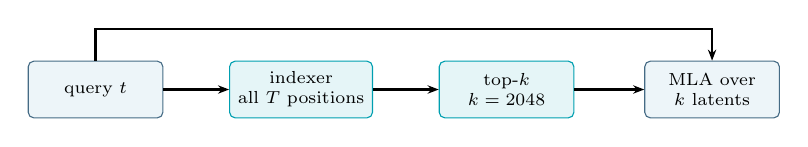
\begin{tikzpicture}[scale=.9,transform shape,every node/.style={font=\scriptsize,align=center},
    box/.style={draw=themebluedraw,fill=themebluebg,rounded corners=2pt,minimum height=.8cm,minimum width=1.9cm},
    cheap/.style={draw=accentdarkdraw,fill=accentdarkbg,rounded corners=2pt,minimum height=.8cm,minimum width=1.9cm},
    arr/.style={-{Stealth[length=4pt]},thick}]
    \node[box] (q) at (0,0) {query $t$};
    \node[cheap] (idx) at (2.9,0) {indexer\\all $T$ positions};
    \node[cheap] (top) at (5.8,0) {top-$k$\\$k=2048$};
    \node[box] (mla) at (8.7,0) {MLA over\\$k$ latents};
    \draw[arr] (q)--(idx); \draw[arr] (idx)--(top); \draw[arr] (top)--(mla);
    \draw[arr] (q.north) -- ++(0,.45) -| (mla.north);
  \end{tikzpicture}
  \par\vspace{6pt}
  \[
    I_{t,s}=\sum_{j=1}^{H^I} w_{t,j}\,\operatorname{ReLU}\!\big(q^{I}_{t,j}\cdot k^{I}_{s}\big),
    \qquad
    \mathcal{S}_t=\operatorname{top-}k_s\,I_{t,s}
  \]
  \small
  \begin{tabular}{@{}lcc@{}}
    \toprule
    Per layer & dense MLA & MLA + DSA \\
    \midrule
    attention, per query & $\mathcal{O}(T)$ & $\mathcal{O}(k)$ \\
    indexer, per query & --- & $\mathcal{O}(T)$, cheap per pair \\
    extra cache per token & --- & one indexer key (128 values) \\
    \bottomrule
  \end{tabular}
  \smallsource{DeepSeek-V3.2 (2025); $H^I=32$ heads of width 128 in all three models}
\end{frame}

\begin{frame}{Why DSA pays even though the indexer is still $\mathcal{O}(T)$}
  \small
  Multiply--adds for one query--key pair, Mistral Large 4 shapes, absorbed MLA:
  \par\vspace{6pt}
  \centering
  \begin{tabular}{@{}lrr@{}}
    \toprule
    & per head & all heads \\
    \midrule
    MLA: score ($512+64$) and value ($512$) & 1088 & $64\times1088\approx70$k \\
    Indexer: $32$ heads $\times\,128$ & 128 & $\approx4$k \\
    \bottomrule
  \end{tabular}
  \par\vspace{8pt}
  \raggedright
  \begin{itemize}
      \setlength{\itemsep}{4pt}
    \item About $17\times$ less work per pair, often in FP8, on all $T$ positions.
    \item Full attention only on $k=2048$ of them.
    \item Prefill keeps an $\mathcal{O}(T^2)$ indexer term: cheaper per pair, not sub-quadratic.
  \end{itemize}
  \begin{alertblock}{Trained in, not switched on}
    \small DeepSeek first trains the indexer to match dense attention, then continues training with sparse selection.
  \end{alertblock}
\end{frame}

\begin{frame}{Kimi Delta Attention: a fixed-size state per head}
  \small
  \[
    S_t=\big(I-\beta_t\,k_tk_t^{\top}\big)\operatorname{Diag}(\alpha_t)\,S_{t-1}+\beta_t\,k_t v_t^{\top},
    \qquad
    o_t=S_t^{\top}q_t,
    \qquad S_t\in\mathbb{R}^{d_k\times d_v}
  \]
  \begin{columns}[t]
    \begin{column}{0.52\linewidth}
      \footnotesize
      \begin{itemize}
          \setlength{\itemsep}{2pt}
        \item $\alpha_t\in(0,1)^{d_k}$: forget gate \textbf{per channel}. Gated DeltaNet uses one scalar per head.
        \item $\beta_t$: write strength; $(I-\beta_tk_tk_t^{\top})$ erases what was stored along $k_t$.
        \item Training: chunk-wise parallel kernels, so mostly matmuls.
      \end{itemize}
    \end{column}
    \begin{column}{0.44\linewidth}
      \begin{block}{Cost model}
        \footnotesize
        State per layer: $H\,d_k\,d_v$ numbers, independent of $T$.\par
        GLM-5.3-Flash: $64\times128\times128\times4$\,B $=4$\,MiB per layer (FP32).
      \end{block}
    \end{column}
  \end{columns}
  \vspace{-2pt}
  \begin{alertblock}{Fixed size is not unlimited memory}
    \footnotesize The state keeps what fits in $d_k\times d_v$ numbers per head. Exact retrieval of an arbitrary old token needs attention layers.
  \end{alertblock}
  \vspace{-6pt}\hfill{\tiny\color{neutraldark}Source: Kimi Linear (2025); Gated Delta Networks (2024)}
\end{frame}

\begin{frame}{mHC: four residual streams, mixed under a constraint}
  \centering
  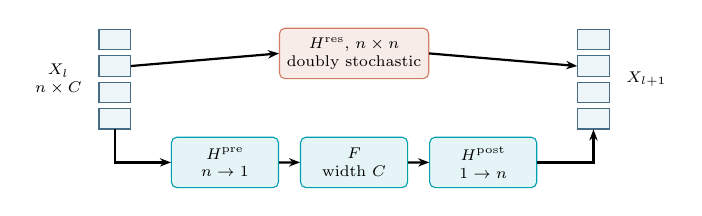
\begin{tikzpicture}[scale=.8,transform shape,every node/.style={font=\scriptsize,align=center},
    stream/.style={draw=themebluedraw,fill=themebluebg,minimum width=.5cm,minimum height=.32cm},
    blk/.style={draw=accentdarkdraw,fill=accentdarkbg,rounded corners=2pt,minimum width=1.7cm,minimum height=.8cm},
    arr/.style={-{Stealth[length=4pt]},thick}]
    \foreach \k in {0,1,2,3}{\node[stream] (a\k) at (0,1.2-.42*\k) {}; \node[stream] (b\k) at (7.6,1.2-.42*\k) {};}
    \node[anchor=east] at (-.4,.57) {$X_l$\\$n\times C$};
    \node[anchor=west] at (8.0,.57) {$X_{l+1}$};
    \node[blk] (pre) at (1.75,-.75) {$H^{\text{pre}}$\\$n\to1$};
    \node[blk] (f) at (3.8,-.75) {$F$\\width $C$};
    \node[blk] (post) at (5.85,-.75) {$H^{\text{post}}$\\$1\to n$};
    \node[blk,fill=leafredbg,draw=leafreddraw] (res) at (3.8,.98) {$H^{\text{res}}$, $n\times n$\\doubly stochastic};
    \draw[arr] (a3.south)|-(pre.west); \draw[arr] (pre)--(f); \draw[arr] (f)--(post); \draw[arr] (post.east)-|(b3.south);
    \draw[arr] (a1.east)--(res.west); \draw[arr] (res.east)--(b1.west);
  \end{tikzpicture}
  \par\vspace{4pt}
  \[
    X_{l+1}=H^{\text{res}}_l X_l+\big(H^{\text{post}}_l\big)^{\top}F\big(H^{\text{pre}}_l X_l\big)
  \]
  \small\raggedright
  \begin{itemize}
      \setlength{\itemsep}{3pt}
    \item Sinkhorn iterations make $H^{\text{res}}$ doubly stochastic, so mixing cannot amplify the signal across depth.
    \item GLM-5.3-Flash: $n=4$, 20 Sinkhorn iterations. Reported cost about $6.7\%$ training time.
    \item Systems cost: each token carries a $4\times$ wider residual state between blocks.
  \end{itemize}
  \vspace{-4pt}\hfill{\tiny\color{neutraldark}Source: Hyper-Connections (2024); mHC (2025)}
\end{frame}

\checkpoint{the price of DSA}
{DSA still has an $\mathcal{O}(T^2)$ term in prefill. Give two reasons it can still be worth training a model with it.}

\begin{frame}{The price of DSA: one possible answer}
  \begin{itemize}
      \setlength{\itemsep}{8pt}
    \item \textbf{Constant factor:} the quadratic term runs at about 4k multiply--adds per pair, often FP8, instead of about 70k.
    \item \textbf{Decode:} attention reads $k=2048$ latents per layer, not $T$; only the small indexer keys are scanned.
    \item \textbf{What it does not do:} the cache still grows with $T$, and the indexer scan becomes the next per-request term to reduce.
  \end{itemize}
\end{frame}

% ---------------------------------------------------------------- 17 min
\section{Case study: Mistral Large 4}

\begin{frame}{Mistral Large 4: the config}
  \footnotesize
  \begin{tabular}{@{}>{\ttfamily}l l l@{}}
    \toprule
    \normalfont Field & Value & Reading \\
    \midrule
    hidden\_size, layers & 6144, 72 & \\
    kv\_lora\_rank, qk\_rope\_head\_dim & 512, 64 & 576 cached elements \\
    index\_topk & 2048 & DSA in all 72 layers \\
    indexer\_types & 44 full, 28 shared & reuse the previous selection \\
    kv\_source\_layers & 63 distinct & 39, 43, \ldots, 71 read layer 35 \\
    no\_rope\_layers & 18 NoPE & one layer in four \\
    n\_routed\_experts, top-$k$ & 128, 4 (+1 shared) & softmax router \\
    moe\_intermediate\_size & 6144 & $\approx113$M per expert \\
    final\_logit\_softcapping & 30 & \\
    vocab, context & 204,800, $2^{20}$ & \\
    \bottomrule
  \end{tabular}
  \par\vspace{8pt}
  \small Counting from these fields: $\approx1.05$T total, $\approx52$B active per token ($\approx50$B without embeddings and output layer).
  \smallsource{\texttt{config.json}, Hugging Face; FP8 block-scaled checkpoint}
\end{frame}

\begin{frame}{Two different kinds of sharing}
  \begin{columns}[t]
    \begin{column}{0.48\linewidth}
      \begin{block}{Indexer sharing: the selection}
        \small
        A \texttt{shared} layer attends to the same 2048 positions as the latest \texttt{full} layer, with its own queries and its own latents.\par\vspace{4pt}
        \textbf{Saves:} the $\mathcal{O}(T)$ indexer scan and the indexer keys in 28 layers.
      \end{block}
    \end{column}
    \begin{column}{0.48\linewidth}
      \begin{exampleblock}{KV sharing: the cache}
        \small
        Nine NoPE layers (39, 43, \ldots, 71) write no latent. They attend over layer 35's cache, also NoPE.\par\vspace{4pt}
        \textbf{Saves:} $9\times1152$ B per token, $12.5\%$ of the latent.
      \end{exampleblock}
    \end{column}
  \end{columns}
  \vfill
  \small The KV-sharing layers keep their own indexers: the two mechanisms are independent.\par
  \vspace{4pt}
  \footnotesize\textcolor{inkmuted}{Neither Mistral nor vLLM states why these choices were made; the savings above are what the config implies.}
\end{frame}

\begin{frame}{Cache per token, and what remains at $T=2^{20}$}
  \small
  BF16 latent, FP8 indexer key (128\,B + 4\,B scale, as in vLLM):
  \[
    \underbrace{63\times576\times2}_{72{,}576\ \text{B}}
    +\underbrace{44\times132}_{5{,}808\ \text{B}}
    =78{,}384\ \text{B}\approx76.5\ \text{KiB per token}
  \]
  One request at $T=2^{20}$: \textbf{$\approx77$ GiB}. With an FP8 latent, vLLM reports 47,136 B per token.
  \par\vspace{8pt}
  Per decode step and request at $T=2^{20}$:
  \par\vspace{4pt}
  \centering
  \begin{tabular}{@{}lr@{}}
    \toprule
    sparse attention: $63\times2048\times1152$ & $0.15$ GB \\
    indexer scan: $44\times2^{20}\times132$ & $\mathbf{6.1}$ \textbf{GB} \\
    active weights (FP8), shared by the batch & $\approx52$ GB \\
    \bottomrule
  \end{tabular}
  \begin{alertblock}{The next bottleneck}
    \small At long context and large batch, the indexer scan dominates per-request traffic. Indexer sharing reduces exactly this term.
  \end{alertblock}
\end{frame}

% ---------------------------------------------------------------- 18 min
\section{Case study: GLM-5.2 to GLM-5.3-Flash}

\begin{frame}{Same MoE recipe, three of four attention layers replaced}
  \footnotesize
  \begin{tabular}{@{}lll@{}}
    \toprule
    & GLM-5.2 & GLM-5.3-Flash \\
    \midrule
    total / active & 744B / 40B & 320B / 18B \\
    hidden, layers & 6144, 78 (+1 MTP) & 4096, 45 (+1 MTP) \\
    attention & 78 MLA + DSA & 34 KDA + 11 MLA + DSA (\texttt{KKKD}) \\
    $d_c$ / $d_R$ & 512 / 64 & 512 / 0, NoPE \\
    indexer & 21 own, 57 shared & 11 own, pooled by 4 tokens \\
    KDA heads & --- & $64\times128\times128$, conv width 4 \\
    experts & 256, top-8, +1 shared & 288, top-8, +1 shared \\
    expert width & 2048 & 2048 \\
    router & sigmoid, bias balancing & same \\
    residual & standard & mHC, 4 streams \\
    vision & --- & native ViT, 24 layers \\
    \bottomrule
  \end{tabular}
  \par\vspace{8pt}
  \small Counting from the config: $\approx313$B + $\approx7$B MTP; $\approx17$--$18$B active.
  \smallsource{\texttt{config.json} files, Hugging Face; Raschka (2026)}
\end{frame}

\begin{frame}{Cache per token against a fixed state}
  \small
  \[
    \text{cache: }\ 11\times512\times2+11\times132=12{,}716\ \text{B}\approx12.4\ \text{KiB per token}
  \]
  \[
    \text{state: }\ 34\times64\times128\times128\times4\ \text{B}=136\ \text{MiB per request (FP32)}
  \]
  \centering
  \begin{tabular}{@{}rrr@{}}
    \toprule
    $T$ & Mistral Large 4 & GLM-5.3-Flash (cache + state) \\
    \midrule
    4k & 0.30 GiB & 0.18 GiB \\
    32k & 2.4 GiB & 0.52 GiB \\
    128k & 9.6 GiB & 1.7 GiB \\
    $2^{20}$ & 76.5 GiB & 12.5 GiB \\
    \bottomrule
  \end{tabular}
  \par\vspace{6pt}
  \raggedright
  GLM-5.2 for comparison: $\approx90.5$ KiB per token.
  \begin{alertblock}{Crossover near 11k tokens}
    \small Below it, most per-request memory is fixed state. Short-prompt, high-concurrency serving gains much less than the 1M headline suggests.
  \end{alertblock}
\end{frame}

\begin{frame}{Why keep eleven attention layers?}
  \begin{columns}[t]
    \begin{column}{0.48\linewidth}
      \begin{block}{What they provide}
        \small
        \begin{itemize}
            \setlength{\itemsep}{3pt}
          \item Exact access to any earlier token; the KDA state is a summary.
          \item NoPE is enough: KDA already encodes order.
          \item Only 11 indexers, scoring pools of 4 tokens: a much smaller $\mathcal{O}(T)$ scan.
        \end{itemize}
      \end{block}
    \end{column}
    \begin{column}{0.48\linewidth}
      \begin{alertblock}{What the design costs}
        \small
        \begin{itemize}
            \setlength{\itemsep}{3pt}
          \item Lossy memory in 34 layers: ask for retrieval-heavy evaluations, not perplexity.
          \item Two layer types to fuse, shard and serve.
          \item Context parallelism passes a state between ranks instead of K/V blocks (M8).
          \item $4\times$ wider residual (mHC).
        \end{itemize}
      \end{alertblock}
    \end{column}
  \end{columns}
  \vfill
  \footnotesize\textcolor{inkmuted}{Pooling by 4 tokens is read from the config and the Transformers code; Z.ai has not described it.}
\end{frame}

\checkpoint{crossover}
{A service runs GLM-5.3-Flash with 4k-token chats at 200 concurrent requests. Another runs 512k-token code-base queries, 4 at a time. For which one does the hybrid design save more memory over Mistral Large 4's scheme, and roughly by how much?}

\begin{frame}{Crossover: one possible answer}
  \small
  Per request, from the cost model:
  \par\vspace{4pt}
  \centering
  \begin{tabular}{@{}lrrr@{}}
    \toprule
    & per request, ML4 & per request, GLM-5.3 & total ratio \\
    \midrule
    4k, 200 requests & 0.30 GiB & 0.18 GiB & $\approx1.6\times$ \\
    512k, 4 requests & 38.3 GiB & 6.3 GiB & $\approx6\times$ \\
    \bottomrule
  \end{tabular}
  \par\vspace{8pt}
  \raggedright
  \begin{itemize}
      \setlength{\itemsep}{5pt}
    \item Short contexts: the fixed 136 MiB state dominates GLM-5.3's footprint.
    \item Long contexts: only the 11 latent layers grow, so the ratio approaches $76.5/12.4\approx6$.
    \item Compare cache layouts, not model quality: these are different models.
  \end{itemize}
\end{frame}

% ---------------------------------------------------------------- side by side
\begin{frame}{Side by side}
  \footnotesize
  \begin{tabular}{@{}>{\raggedright\arraybackslash}p{.27\linewidth}>{\raggedright\arraybackslash}p{.31\linewidth}>{\raggedright\arraybackslash}p{.33\linewidth}@{}}
    \toprule
    & Mistral Large 4 & GLM-5.3-Flash \\
    \midrule
    main idea & every layer sparse; share selections and caches & most layers recurrent; the rest sparse \\
    cache per token & $\approx76.5$ KiB & $\approx12.4$ KiB + 136 MiB fixed \\
    per-request scan & indexer, 44 layers & indexer, 11 layers, pooled \\
    experts & 128, top-4, $d_{ff}=6144$ & 288, top-8, $d_{ff}=2048$ \\
    dispatch, BF16 & $4\times6144\times2=48$ KiB & $8\times4096\times2=64$ KiB \\
    FLOPs per byte sent & $\approx18$k & $\approx6$k \\
    position & 3:1 RoPE : NoPE & NoPE; order from KDA \\
    \bottomrule
  \end{tabular}
  \par\vspace{2pt}
  {\scriptsize\textcolor{inkmuted}{Dispatch: per token and MoE layer. FLOPs: routed-expert FLOPs per dispatched byte.}}
  \par\vspace{4pt}
  \small
  \begin{block}{Module 8 connection}
    Fine-grained experts give more expert combinations per token, but less compute for each byte sent through All-to-All. That communication is harder to hide.
  \end{block}
\end{frame}

% ---------------------------------------------------------------- 15 min
\section{Exercise: read an unknown config}

\begin{frame}{Model X (invented for this exercise)}
  \footnotesize
  \begin{tabular}{@{}ll@{}}
    \toprule
    hidden\_size & 5120 \\
    layers & 48, pattern \texttt{GGGM} (G: gated DeltaNet, M: MLA) \\
    MLA & $d_c=512$, $d_R=64$, dense (no indexer) \\
    linear layers & 40 heads, $d_k=d_v=128$, FP32 state \\
    MoE & 256 routed, top-8, 1 shared, $d_{ff}=1536$ \\
    dense layers before MoE & 2, $d_{ff}=12288$ \\
    vocabulary & 160,000, untied embeddings \\
    attention and recurrent projections & 6.0B parameters in total (given) \\
    \bottomrule
  \end{tabular}
  \par\vspace{6pt}
  \small
  \begin{enumerate}
      \setlength{\itemsep}{2pt}
    \item KV-cache bytes per token in BF16.
    \item Recurrent state per request.
    \item Crossover context, and the per-request total at 128k.
    \item Total and active parameters (a SwiGLU expert has $3\,C\,d_{ff}$).
    \item Which cost does it target? What evidence would you ask for?
  \end{enumerate}
\end{frame}

\begin{frame}{Model X: one possible answer}
  \small
  \begin{enumerate}
      \setlength{\itemsep}{4pt}
    \item $12\times576\times2=13{,}824$ B $=13.5$ KiB per token (all-MLA: 54 KiB).
    \item $36\times40\times128\times128\times4$ B $=90$ MiB.
    \item $90\ \text{MiB}/13.5\ \text{KiB}\approx6.8$k tokens. At 128k: $1.69+0.09\approx1.8$ GiB (all-MLA: 6.75 GiB).
    \item Expert: $3\times5120\times1536\approx23.6$M. MoE: $46\times257\times23.6\text{M}\approx279$B total, $46\times9\times23.6\text{M}\approx9.8$B active. Add dense $0.38$B, embeddings $1.64$B, projections $6.0$B: $\approx$\,\textbf{287B total}, $\approx$\,\textbf{17.8B active}.
    \item Per-request memory and bandwidth at long context. Ask for multi-needle and multi-hop retrieval against an all-attention baseline trained the same way, and measured decode throughput against context length.
  \end{enumerate}
\end{frame}

\takeaways
{A config is a list of cost decisions: read the layer pattern, cached elements, indexer and expert fields before the benchmark table.}
{DSA makes attention $\mathcal{O}(k)$ per query but keeps a cheap $\mathcal{O}(T)$ scan; sharing selections and caches targets what remains.}
{Hybrid recurrence trades a growing cache for a fixed state: compute the crossover before claiming a memory win.}
{Every saving moves the bottleneck: indexer scans, fixed state, wider residuals, All-to-All per FLOP.}

\begin{frame}{Sources}
  \footnotesize
  \begin{itemize}
      \setlength{\itemsep}{3pt}
    \item Mistral Large 4: \texttt{config.json}; Hugging Face release post; vLLM day-0 post (Oct.\ 2026).
    \item GLM-5.3-Flash and GLM-5.2: \texttt{config.json}; Transformers \texttt{glm5\_next} docs; Raschka, \emph{GLM-5.3-Flash architecture notes} (Aug.\ 2026).
    \item GLM-5 technical report (2026): DSA in the GLM-5 family.
    \item DeepSeek-V3.2 (2025): DeepSeek Sparse Attention.
    \item Kimi Linear (2025); Gated Delta Networks (2024).
    \item Hyper-Connections (2024); mHC (2025).
    \item DeepSeek-V2 (2024): multi-head latent attention.
  \end{itemize}
  \vfill
  \small Parameter and byte counts are computed from the configs. Cache sizes depend on the implementation: state your convention.
\end{frame}

\end{document}
